\chapter{Design e scelte implementative}

\section{Server}

Come gi\`a specificato nei precedenti capitoli, il Server deve esporre verso l'esterno due interfacce: l'interfaccia REST e l'interfaccia Web. Lo scopo della prima \`e quello di fornire un'interfaccia che consenta a un utente di poter:
\begin{itemize}
	\item Ricevere la lista di tutte le griglie presenti sul Server;
	\item Visualizzare una particolare griglia tra quelle disponibili;
	\item Richiedere un cammino minimo fra due nodi di una particolare griglia.
\end{itemize}
Per l'interfaccia Web, invece, \`e previsto che questa debba permettere all'utente di:
\begin{itemize}
	\item Inserire una griglia nel database;
	\item Visualizzare tutte le griglie salvate nel database;
	\item Eliminare una griglia dal database.
\end{itemize}
Entrambe le interfacce fanno uso di un'interfaccia interna all'applicazione: l'interfaccia \emph{IGridService}. Questa interfaccia ha il compito di fornire le operazioni necessarie per svolgere la funzione prevista dal sistema, ossia chi usa IGridService non vede i dettagli implementativi riguardanti come le operazioni di lettura e scrittura sul database vengono effettivamente realizzate. IGridService fornisce inoltre l'operazione di ricerca del cammino minimo, i cui dettagli verranno spiegati in seguito.\\*
IGridService viene estesa da una classe concreta (ConcreteGridService) che implementa direttamente l'algoritmo di ricerca del cammino minimo, delegando tutte le operazioni relative alla lettura e scrittura dal e sul database all'interfaccia IMongoRepository<DatabaseGrid,String>, estensione della generica interfaccia di Spring Boot MongoRepository<T,S>. Questa interfaccia definisce la mappatura tra oggetti DatabaseGrid salvati sul database e le stringhe ID che li identificano, mentre l'implementazione dei metodi di lettura e scrittura \`e definita dal bean iniettato dal framework a run-time (il quale \`e disponibile di default).\\*
L'intero sviluppo del sistema client-server ha seguito la metodologia test-driven.\\*
Nei classici modelli di sviluppo software a cascata, o a V, prima di poter scrivere il codice \`e necessario definire i requisiti funzionali e non funzionali del sistema da implementare, e i successivi test hanno lo scopo di verificare che il comportamento del sistema sia coerente rispetto ai requisiti derivati dall'analisi effettuata a priori. Solo dopo aver verificato che un certo sistema soddisfi le propriet\`a imposte dai requisiti pu\'o seguire il processo di \emph{validazione}. In tale fase, lo scopo \`e quello di validare un sistema sulla base delle funzionalit\`a attese dal cliente/committente.  Lo sviluppo test-driven accoppia le fasi di analisi dei requisiti e implementazione del codice, infatti scrivere i test prima del codice significa definire il requisito sotto forma di codice Java, e poi realizzare qualcosa che possa soddisfare il requisito appena definito. In quest'ottica, i test case che abbiamo scritto rappresentano altres\`i la definizione di \emph{tutti} i requisiti funzionali del sistema implementato.
\subsection{Rappresentazione delle griglie}
Un oggetto griglia salvato nel database, viene visto dall'interfaccia IGridService come un'istanza della classe \emph{DatabaseGrid}. Questa classe \`e un wrapper di una matrice di interi, la quale rappresenta il grafo. La classe DatabaseGrid aggiunge inoltre informazioni su una griglia associando ad essa un intero (id) e un intero n che rappresenta il numero massimo di righe e colonne che devono essere lette dalla matrice wrappata per estrapolarne la griglia.\\*
Nonostante questa scelta sembra perdere di generalit\`a, in quanto considera solamente matrici quadrate, in realt\`a se volessimo rappresentare una griglia che non sia in generale quadrata, sarebbe sufficiente porre a $0$ le righe o le colonne che non si vuole facciano parte del grafo.\\*
\subsection{REST Controller}
Il REST Controller che abbiamo realizzato \`e una classe, opportunamente annotata secondo la struttura di Spring Boot, che a run-time serve determinate richieste HTTP su tre particolari URL:
\begin{itemize}
	\item /api/ $\rightarrow$ restituisce al client una lista JSON di stringhe rappresentanti ciascun ID delle griglie salvate nel database.
	\item /api/grid$[i]$ $\rightarrow$ restituisce al client l'oggetto griglia avente id='i'  (serializzato come oggetto JSON);
	\item /api/path$[SOURCE]$TO$[SINK]$IN$[ID]$ $\rightarrow$ restituisce al client una lista JSON di stringhe rappresentanti i nodi che fanno parte del cammino minimo nel grafo con id='ID' partendo dal nodo 'SOURCE' e finendo nel nodo 'SINK'. Se il cammino non esiste, viene restituita una lista vuota.
\end{itemize}
La sintassi di un nodo, affinch\`e sia interpretabile dal server, deve rispettare la seguente espressione regolare:
$$
[0-9]^+\texttt{\_}[0-9]^+
$$
La prima cifra rappresenta l'indice di riga del nodo che si vuole considerare, mentre la seconda rappresenta l'indice di colonna.
\subsection{Web Controller}
Al Web Controller sono delegate le operazioni di aggiunta e rimozione di griglie all'interno del database. Tali operazioni sono concesse solo previa autenticazione con username e password. Per implementare il login abbiamo utilizzato la classe WebSecurityConfig, che comunica al framework di abilitare il sistema di login nativo di Spring Boot, escludendo da esso gli URL relativi all'interfaccia REST e permettendo l'accesso a qualsiasi altro URL solamente se identificati con nome utente "user" e password "password".\\*
Gli URL serviti dal Web Controller sono:
\begin{itemize}
	\item / $\rightarrow$ dalla root si accede a una pagina mediante la quale il client sceglie un particolare servizio del Web Controlller;

	
	\item /viewdb $\rightarrow$ viene renderizzata una pagina HTML nella quale sono riportate tutte le griglie presenti nel database;

	\item /addtable $\rightarrow$ viene renderizzata una pagina HTML che prevede l'immissione tramite un form di una griglia all'interno del database;
	
	\item /remtable $\rightarrow$ come addtable, ma il form richiede solo l'inserimento dell'id della griglia che si intende cancellare.
\end{itemize}
\newpage
	\begin{figure}[ht]
	\centering
	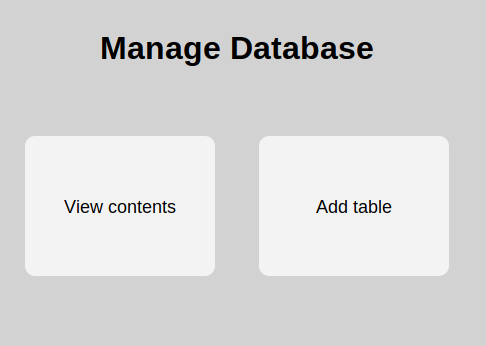
\includegraphics[width=0.7\linewidth]{Images/home}
	\caption{Home page della web-app}
	\label{fig:home}
\end{figure}
	\begin{figure}[ht]
	\centering
	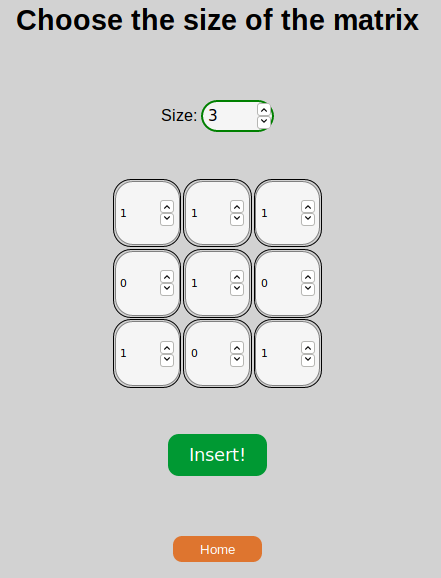
\includegraphics[width=0.7\linewidth]{Images/addtable}
	\caption{Form per l'inserimento di una nuova griglia}
	\label{fig:home}
\end{figure}
	\begin{figure}[ht]
	\centering
	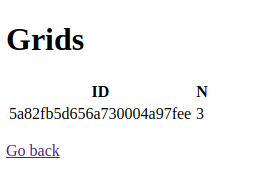
\includegraphics[width=0.7\linewidth]{Images/viewgrids}
	\caption{Lista delle griglie salvate nel database}
	\label{fig:home}
\end{figure}
	\begin{figure}[ht]
	\centering
	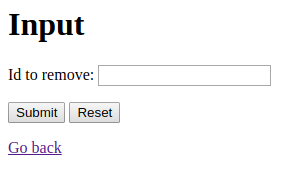
\includegraphics[width=0.7\linewidth]{Images/rem}
	\caption{Form per il cancellamento di una griglia}
	\label{fig:home}
\end{figure}
\newpage
\subsection{Algoritmo di ricerca del cammino minimo}
Per implementare la ricerca del cammino minimo in una griglia rappresentata dalla matrice A, la classe concreta che implementa IGridService (ConcreteGridService) opera nel modo seguente:
\begin{itemize}
	\item Per ogni nodo i,j di A tale che $A[i][j]>0$ aggiungi il nodo i,j a una lista \emph{nodes} di stringhe nella forma 	'$\texttt{i\_j}$';
	\item Per ogni nodo n di nodes:
	\begin{itemize}
		\item Controlla quali vicini ha n (controllando gli indici di riga e colonna come specificato nel capitolo 1)
		\item Se n ha un vicino n', allora aggiungi a una lista \emph{edges} di vettori di stringhe, l'arco $n\rightarrow n'$, dove ciascun arco e \`e un vettore di dimensione 2 tale per cui e$[0]=n$ ed e$[1]=n'$.
	\end{itemize}
\end{itemize}
A questo punto il grafo \`e completamente rappresentato dalla lista dei suoi nodi e dalla lista suoi archi, ed \`e possibile applicarvi il seguente algoritmo di visita per ricercare il cammino minimo tra due nodi source e sink.
\scriptsize
\begin{lstlisting}
Algoritmo cammino_minimo(source,sink):
	crea nodi_visitati;
	crea nodi_precedenti;
	crea lista_cammino_minimo;
	crea coda;
	Nodo corrente=source;
	coda.add(corrente);
	nodi_visitati.add(corrente,true);
	fintantoche(coda non vuota)
		corrente=coda.remove();
		se corrente==sink allora 
			esci;
		altrimenti
			per ogni nodo v vicino di current:
				se nodi_visitati non contiene v:
					coda.add(corrente);
					nodi_visitati(v,true);
					nodi_precedenti.add(v,corrente);
				fine se
			fine per
		fine se
	fine fintantoche
	se corrente != sink allora:
		restituisci lista vuota;
	altrimenti
		per Nodo n=sink, se n non nullo, n=nodi_precedenti.get(n):
			lista_cammino_minimo.add(n);
		fine per
		restituisci reverse(lista_cammino_minimo);
	fine se
fine algoritmo
\end{lstlisting}
\normalsize
\section{Client}
Il Client utilizza l'interfaccia IClient per colloquiare con l'interfaccia REST del Server. Questa classe utilizza al suo interno un'altra interfaccia, IRestServiceClient. Quest'ultima utilizza il framework Apache Http Client col fine di eseguire richieste HTTP sui particolari URL dell'interfaccia REST del Server che abbiamo realizzato. L'interfaccia IClient permette all'utente di:
\begin{itemize}
	\item ricevere la lista di tutte le griglie presenti sul database del Server;
	\item ricevere una particolare griglia;
	\item ricevere un particolare cammino minimo all'interno di una griglia.
\end{itemize}
Gli oggetti ricevuti sono stringhe JSON nel primo e nel terzo caso, mentre quando si riceve una particolare griglia, se ne riceve la serializzazione JSON. Una griglia serializzata tramite JSON viene poi caricata in memoria come un'istanza della classe GridFromServer; classe del tutto equivalente alla classe DatabaseGrid che abbiamo discusso in 3.1.1.
\subsection{Interfaccia utente}
L'applicazione mette a disposizione dell'utente la seguente interfaccia grafica per fare uso di un'implementazione concreta di IClient.
\begin{figure}[ht]
	\centering
	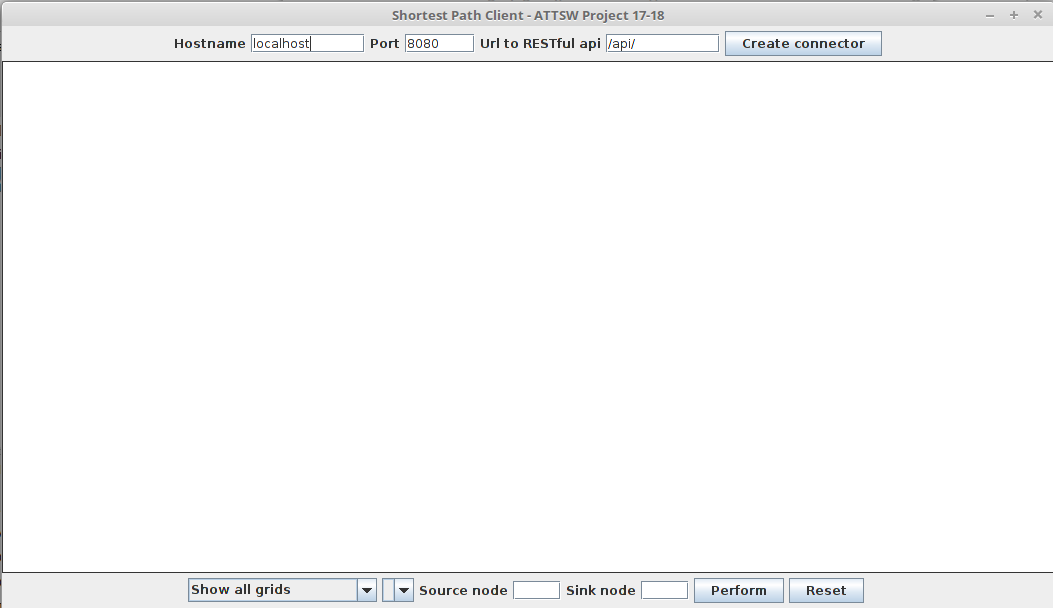
\includegraphics[width=0.7\linewidth]{Chapters/1}
	\caption[Interfaccia utente]{Interfaccia del Client all'avvio del sistema}
	\label{fig:1}
\end{figure}

\begin{figure}[ht]
	\centering
	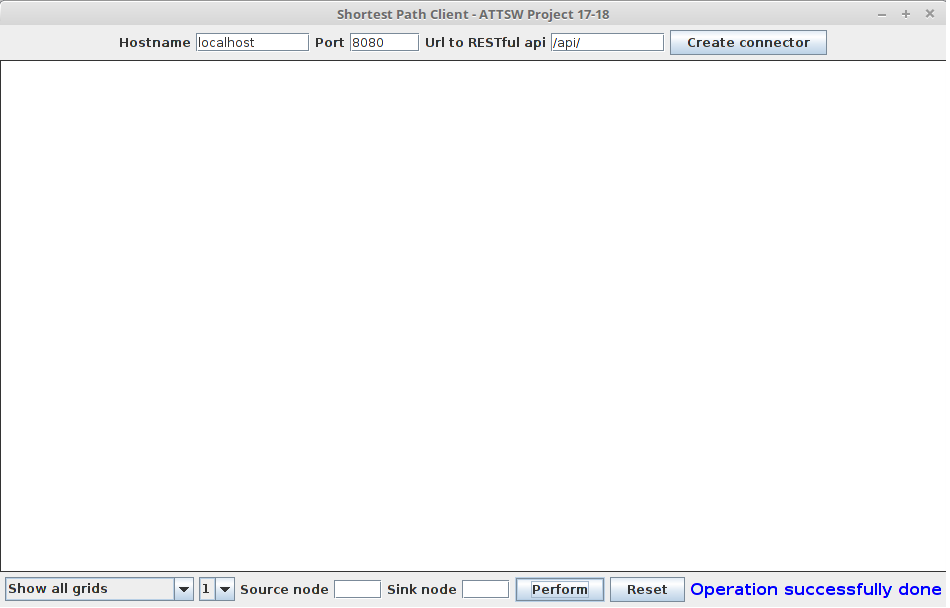
\includegraphics[width=0.7\linewidth]{Chapters/2}
	\caption[Interfaccia utente]{Richiedi tutte le griglie al Server}
	\label{fig:2}
\end{figure}

\begin{figure}[ht]
	\centering
	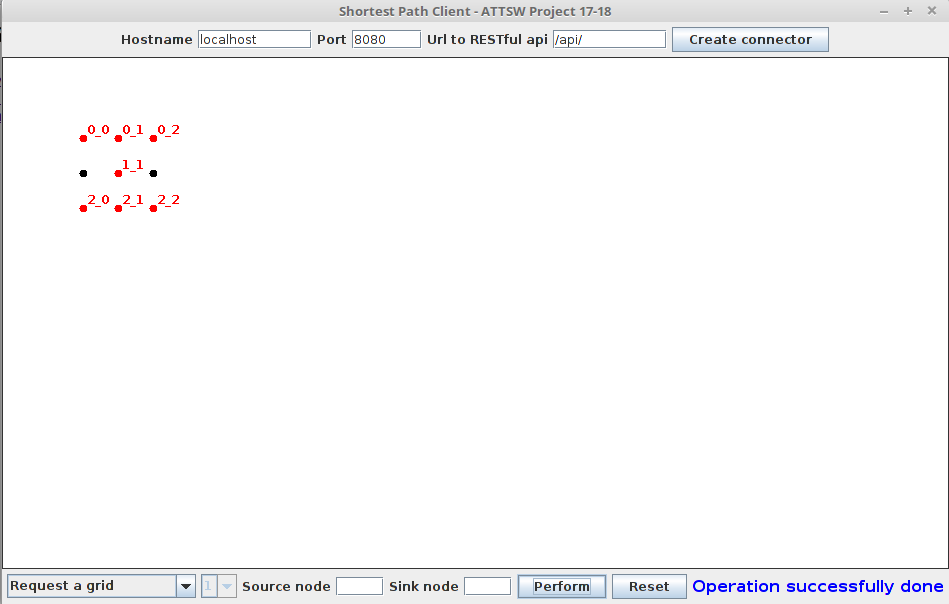
\includegraphics[width=0.7\linewidth]{Chapters/3}
	\caption[Interfaccia utente]{Richiedi griglia con id=1}
	\label{fig:3}
\end{figure}

\begin{figure}[ht]
	\centering
	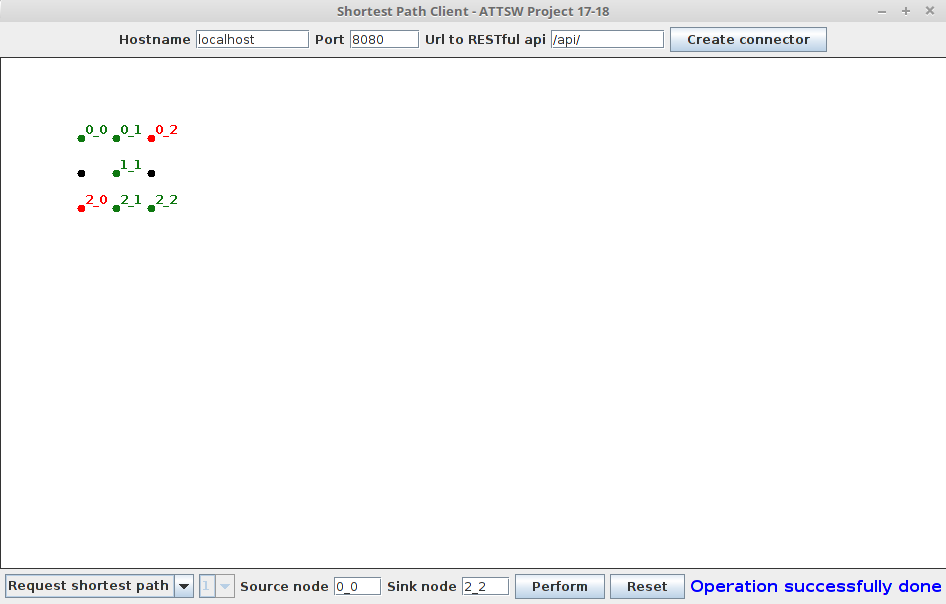
\includegraphics[width=0.7\linewidth]{Chapters/4}
	\caption[Interfaccia utente]{Richiedi il cammino minimo nella griglia 1 da 0,0 a 2,2}
	\label{fig:4}
\end{figure}

 \subsubsection{Implementazione dell'interfaccia}
 L'interfaccia fa uso del framework Swing. Essa \`e gestita da una classe GUI che ha al suo interno un'istanza di JFrame, una classe di Swing che rappresenta una finestra come comunemente intesa dall'utente. Come visto in precedenza, il frame \`e diviso in tre sezioni:
 \begin{itemize}
 	\item NORTH
 	\item CENTER
 	\item SOUTH
 \end{itemize}
A ciascuna di questa sezione corrisponde un JPanel. JPanel \`e una classe di Swing che funziona come container di componenti come pulsanti, barre di inserimento testuale, men\`u, ecc. La classe JPanel pu\`o essere estesa col fine di riscrivere il suo metodo \emph{paintComponent(Graphics g)}, il metodo delegato al disegno del container. Questo \`e quanto avviene per il JPanel corrispondente al centro della finestra; infatti quest'ultimo \`e un'istanza della classe GUIpanel e rappresenta il punto centrale di tutta l'interfaccia grafica realizzata.\\*
Un GUIpanel \`e un oggetto che ha al suo interno una matrice di punti indicizzati (ciascun punto \`e istanza della classe Point del medesimo framework) che possono essere creati e disegnati con differenti colori. Questa struttura si adatta al nostro sistema in quanto per visualizzare una griglia, oppure un cammino al suo interno, \`e sufficiente colorare i punti che fanno parte della griglia rispettivamente di colore rosso e di colore verde. I punti che non fanno parte della griglia e non sono indicizzati dalla matrice ricevuta dal server verranno disegnati come punti \emph{hidden} ossia dello stesso colore dello sfondo del container, cosicch\`e possano apparire all'utente come nascosti. Infine, i nodi indicizzati dalla matrice ricevuta dal server che non fanno parte della griglia, sono visualizzati come punti di colore nero.



